

\subsection{Cluster-Matching-Based Method For Video Face Recognition}
\label{webmedia}

In this first application, we propose a cluster-matching-based approach for video face recognition where \emph{face clustering} is used to group faces in both the face dataset and in the target video~(video face clustering).
%%
Consequently, classes do not have to be previously known, and the effort spent with annotations is significantly reduced --- as it is done over clusters instead of single images.
%%
Face recognition becomes a task of comparing clusters from the dataset with the ones extracted from images or video sources.
%%
Therefore, our approach is easily scalable.

In our approach we use \emph{face clustering} in an images dataset and in the referenced video. Then, the clusters of the images dataset are labeled. Next, we perform \emph{Cluster Matching} where the clusters from the image dataset and from the video are matched using a heuristic based on clusters distance. Figure \ref{fig:cluster_matching} shows our proposed approach.


\begin{figure*}[!ht]
    \centering
    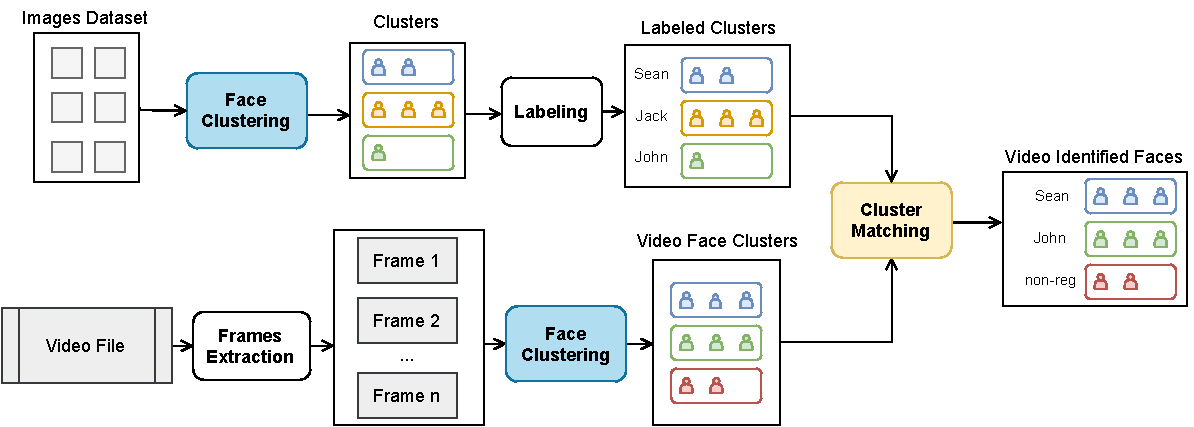
\includegraphics[width=\textwidth]{img/webmedia/cluster_matching_process.pdf}
    \caption{Cluster-Matching based Method for Video Face Recognition.}
    \label{fig:cluster_matching}
\end{figure*}

We have performed two experiments to evaluate our method. 
%%
The first evaluation aimed at measuring how well our approach of \emph{Cluster Matching} performed when clustering images of actors in different occasions~(instead of frames from a video). 
%%
The second evaluation aimed at measuring how well our approach performed on video. Each of these evaluations will be described in details in our dissertation. This application has also been published at a relevant multimedia conference~\cite{mendes2020cluster}.
%%
Figure \ref{fig:timeline_pol} shows an example of our method for video face recognition in a video where two identified Brazilian politicians are shown in each frame with its respective colored cluster.

\begin{figure}[!ht]
    \centering
    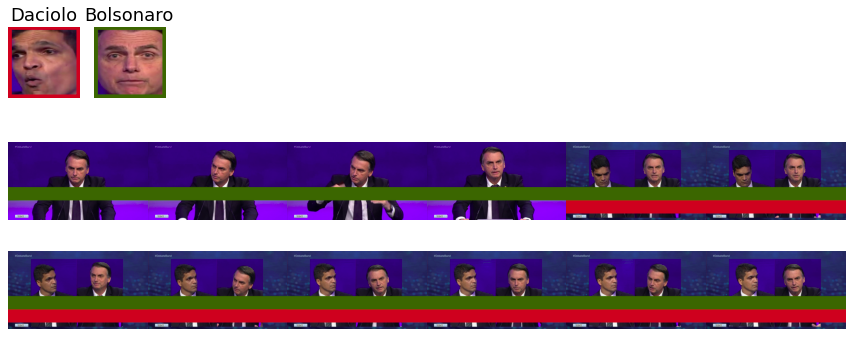
\includegraphics[width=0.6\linewidth]{img/webmedia/timeline_pol.png}
\vspace{-1em}
    \caption{Timeline with tagged frames by their clusters of registered people}
    \label{fig:timeline_pol}
\end{figure}


